% ============================================================
% Restructured Section 3.7 (Effects of Opacity) + Section 3.8 (Implications)
% Response to co-author comments #27 and #33 (2026-04-23 Comments.docx)
%
% Purpose:
%   - Extract "Equilibrium Comparison" out of \subsection{Equilibrium} (3.6)
%   - Create new \subsection{Effects of Opacity} (new 3.7) that unifies:
%       (i) the equilibrium comparison (Corollary cor:high_vs_low)
%      (ii) opacity/trading-style/performance analysis, combining the current
%           \subsubsection{Opacity and Trading Style} (in 3.7 Implications) with
%           the content of \subsection{Opacity as Commitment Device} (in 4.2).
%   - Rename current \subsection{Implications} (3.7) to 3.8, dropping the
%     subsubsection \subsubsection{Opacity and Trading Style} (moved to 3.7.2).
%   - The content itself is unchanged; this is a pure re-ordering / re-sectioning.
%
% HOW TO APPLY THIS FILE
% ----------------------
% 1. In 02_MainBody/023_Equilibrium.tex:
%    (a) Inside \subsection{Equilibrium} (\label{ss:equilibrium}), delete the
%        \subsubsection{Equilibrium Comparison} block and its associated text
%        (currently lines ~149--172), including Corollary cor:high_vs_low and
%        the paragraph-by-paragraph intuition for statements (i)--(v).
%    (b) Delete the entire \subsection{Implications} block (currently
%        lines ~175--242).
%    (c) After the end of \subsection{Equilibrium}, \input{} this file, or
%        paste its content in directly.
%
% 2. In 02_MainBody/024_EndogenousOpacity.tex:
%    (a) Delete the entire \subsection{Opacity as Commitment Device} block
%        (currently lines ~25--43), including equation eq:unconditional pi,
%        Corollary cor:opacity_performance, the input of fig:opacity_pi, equation
%        eq:investor utility, and the paradox/timing paragraph.
%    (b) After \subsection{Setup}, the next subsection now becomes
%        \subsection{Equilibrium Opacity} directly. Consider adding a brief
%        forward-reference sentence to new Section 3.7.2 at its opening, since
%        Corollary cor:opacity_performance (now in 3.7.2) is the basis for the
%        obfuscation incentive.
%
% RELATED COMMENTS STILL PENDING (not addressed here; apply in-line later):
%   #41  Section 4.2 title → N/A (subsection 4.2 is removed by this reorg)
%   #42  Move Corollary 4.1 to Section 3.6 → accomplished (now in 3.7.2 as
%        cor:opacity_performance)
%   #43  "in order to" → "in an attempt to" (in paragraph moved from 4.2)
%   #44  "fund flow compensates for this loss" is factually wrong (same paragraph)
%   #45  "Fund opacity, conversely..." rewrite (same paragraph)
%   #46  investors' ex-ante utility forward-move → accomplished
%   #47  paradox/timing paragraph rewrite (in the 4.2 paragraph moved here)
% ============================================================

%===========================================
\subsection{Effects of Opacity}\label{ss:effects_of_opacity}

\subsubsection{High-\texorpdfstring{$\beta$}{beta} vs.\ Low-\texorpdfstring{$\beta$}{beta} Equilibrium}\label{sss:high_vs_low}
Comparing the two stable equilibria, does the manager perform better in one of them? What are the implications for market liquidity, asset prices, and learning about asset-selection skills?
%The following corollary summarizes the results.
\begin{corollary}[High-$\beta$ vs.\ low-$\beta$ equilibrium]\label{cor:high_vs_low}
In the high-$\beta$ equilibrium, relative to the low-$\beta$ equilibrium, the following results hold.
\begin{enumerate}[label=(\roman*)]
\item \label{item:1} The market is more liquid, that is, $\lambda$ is lower;
\item \label{item:2} The manager's expected investment performance given the realized skill, $\mathrm{E}[(\delta-p)x|s]=\frac{\beta\omega_{u}s^{2}}{\beta^{2} \omega_{s}+\omega_{u}}$, is lower;
\item \label{item:3} The price informativeness, defined by $\tau\equiv\frac{1}{\mathrm{Var}[\delta|p]}=\frac{\beta^{2} \omega_{s}+\omega_{u}}{\omega_{u} \omega_{s}}$, is higher;
\item \label{item:4} The price volatility, $\mathrm{Var}[p]=\frac{\beta^{2}\omega_{s}^{2}}{\beta^{2} \omega_{s}+\omega_{u}}$, is higher; and
\item \label{item:5} Investors' estimate of the manager's skill is more precise, that is, $\hat{\omega}_{s}=\mathrm{Var}[s|f] = \frac{\omega_{s}\omega_{\eta}}{\beta^{2}\omega_{s}+\omega_{\eta}}$ is lower.
\end{enumerate}
\end{corollary}

Statement \ref{item:1} of Corollary \ref{cor:high_vs_low} holds because price impact $\lambda$ is decreasing in $\beta$ in the equilibrium. Namely, the information is exaggerated in that the order size is too large relative to the true $|s|$ due to the showing-off motive. Thus, the market maker attempts to partially ``undo" the manager's information revelation by incorporating less of it into the price, resulting in a weaker price impact.\footnote{$\lambda$ represents the price's reaction to the order flow $x+u$, rather than its reaction to the manager's private information $s$. The price impounds $s$ with coefficient $\beta\lambda$, which is monotonically increasing in $\beta$.} Since the high-$\beta$ equilibrium emerges only if the fund is relatively transparent, the statement also implies that a higher fund transparency leads to higher market liquidity.

The intuition for statement \ref{item:2} is closely related to that for statement \ref{item:1}. In the high-$\beta$ equilibrium, the manager earns a lower trading profit due to a smaller informational advantage over the market maker. This result may appear inconsistent with statement \ref{item:1} because, ceteris paribus, a lower price impact is typically associated with a higher trading profit. However, the manager's order size $|x|$ in the high-$\beta$ equilibrium is so large that the {\it overall} price reaction (i.e., $\lambda$ multiplied by $|x|$) is larger than that in the low-$\beta$ equilibrium. Consequently, the manager moves the price excessively and earns a lower trading profit in this equilibrium.
%\footnote{Our numerical result, not presented in the paper but available upon request, indicates that the trader's overall expected utility, including the reputation benefit, is also lower in the high-$\beta$ equilibrium.}
Due to her aggressive trading, more information about $s$, which is informative about $\delta$, is incorporated into the price in the high-$\beta$ equilibrium, supporting statement \ref{item:3}.

Statement \ref{item:4} follows, again, from the manager's aggressive trading in the high-$\beta$ equilibrium. Specifically, she places a large buy (sell) order when $s>0$ ($s<0$), even if $|s|$ is small. This causes a large upward (downward) pressure on $p$, leading to greater price variability. This result aligns with the insight of \citet{guerrieri2012fund} that reputation concerns amplify price volatility, although their mechanism differs from ours.\footnote{\citet{guerrieri2012fund} argue that bond price volatility increases because fund managers demand a premium to offset the risk of reputation damage in the event of default.}

In the high-$\beta$ equilibrium, the manager reveals more information about $s$, thereby improving the precision of investors' estimation, as statement \ref{item:5} demonstrates. This makes fund flows more responsive to skill, as investors can assess it more accurately.

%-------------------------------------------
\subsubsection{Opacity, Trading Style, and Performance}\label{sss:opacity_style_perf}
Having compared the two stable equilibria at a fixed level of fund opacity, we now examine how fund opacity $\omega_{\eta}$ itself shapes equilibrium trading behavior, fund performance, and investor welfare. These comparative statics establish the economic role of opacity and set the stage for the transparency-backfires result.

\paragraph{\normalfont{\textit{Opacity and trading intensity.}}}
Proposition \ref{prop:eqm} yields novel implications connecting the fund opacity and trading styles.
\begin{corollary}\label{cor:beta opacity}
    Both in the high- and low-$\beta$ equilibria, the trading intensity $\beta$ is monotonically decreasing in the fund opacity $\omega_{\eta}$.
\end{corollary}
Figure \ref{fig:opacitybeta} illustrates the result in Corollary \ref{cor:beta opacity}: the left panel represents the case with a unique equilibrium by setting a weak flow-performance sensitivity, while the right panel involves multiple equilibria due to a strong flow-performance sensitivity.
First, as both panels illustrate, opaque funds tend to adopt low-intensity strategies (i.e., the low-$\beta$ equilibrium) that minimize market impact, prioritizing profits over fund flows. In contrast, transparent funds engage in high-intensity strategies with flashy risk taking (i.e., the high-$\beta$ equilibrium), seeking reputation among investors and large fund flows. This relationship arises because the manager's reputation becomes insensitive to her trading behavior when the fund information is opaque and difficult to interpret for fund investors. The model predicts that these tendencies are more pronounced when the flow-performance sensitivity is weak, as the equilibrium is unique regardless of fund opacity (panel [a] of Figure \ref{fig:opacitybeta}).

\input{Figures/fig_opacity_beta_2}

These results are consistent with common observations in the real market. For example, quantitative hedge funds are often extremely opaque and highly profit-driven, focusing on consistent performance, with benefits from attracting fund flows being regarded as secondary to profitability (\citealp{schwager2012hedge}). On the other hand, some transparent funds, such as certain thematic ETFs or crypto-focused funds, engage in bold, attention-grabbing strategies to attract investor flows. These funds often emphasize visibility and narrative-driven positioning, which can lead to volatile returns and greater risk taking.

The second implication is drawn from the model's multiple equilibria, as panel (b) in Figure \ref{fig:opacitybeta} illustrates. Namely, the relation between funds' activities ($\beta$) and their transparency ($\omega_{\eta}$) becomes indeterminate when the opacity is at an intermediate level. Notably, this indeterminacy may lead to financial fragility. Depending on market beliefs, funds with intermediate opacity may shift between profit-seeking and reputation-driven strategies, creating non-fundamental fluctuations. Our result suggests that even relatively opaque funds may follow the crowd due to market beliefs, switching between safe and risky strategies.

A notable observation in line with this result is momentum crashes (\citealp{daniel2016momentum}), where funds engaging in risky and visible momentum trades often switch to safer strategies, generating sharp reversals and amplifying price declines. More generally, the rapid shifts between risk-taking and solid performance-based behavior have contributed to market fragility and volatility, as documented in various studies on economic crises, such as \citet{brunnermeier2009deciphering} on the Global Financial Crisis in 2007. Importantly, large fundamental shifts that support such transitions are rarely identified (\citealp{gennotte1999market}). Our model does not require such fundamental shocks, as a change in beliefs alone can trigger a shift.

\paragraph{\normalfont{\textit{Opacity and fund performance.}}}
We next turn to the relationship between fund opacity and fund performance. Given the trading intensity $\beta$, the unconditional expectation of fund performance is computed as
\begin{equation}
     \mathrm{E}[\pi] = \frac{\beta \omega_{u}}{\beta^2 \omega_{s} + \omega_{u}}\omega_{s}.\label{eq:unconditional pi}
\end{equation}
As in the standard \citet{kyle1985continuous} framework, the first fraction represents the profit margin that each unit of informational advantage would earn, and the second term $\omega_s$ represents the average magnitude squared of the informational advantage.

Fund opacity $\omega_{\eta}$ does not directly show up in equation \eqref{eq:unconditional pi}, but it influences the expected performance through the equilibrium trading intensity $\beta$, as Corollary \ref{cor:beta opacity} demonstrates.
\begin{corollary}\label{cor:opacity_performance}
     Both in the low- and high-$\beta$ equilibria, the expected fund performance $\mathrm{E}[\pi]$ is monotonically increasing in fund opacity $\omega_{\eta}$.
 \end{corollary}
 \input{Figures/fig_opacity_beta_profit}
 Figure \ref{fig:opacity_pi} plots $\mathrm{E}[\pi]$ in relation to  $\omega_{\eta}$, which traces the reactions of $\beta$ in Figure \ref{fig:opacitybeta}. In our model, holding other parameters fixed, $\mathrm{E}[\pi]$ declines with the trading intensity $\beta$. This arises from the presence of the showing-off motive. Although unconditional expected performance is maximized at the Kyle benchmark, which is driven solely by the hiding motive, the manager in our model trades more aggressively in order to attract fund flows. It reveals too much private information to the market maker and lowers the fund performance, while the manager is willing to deviate from the profit-maximizing strategy because the fund flow compensates for this loss. Fund opacity, conversely, diminishes the showing-off motive and induces the manager to pursue more profit-driven strategies, bringing $\beta$ closer to the profit-maximizing level. As a consequence, opacity helps improve the expected fund performance.

\paragraph{\normalfont{\textit{Investor welfare and transparency backfires.}}}
Interestingly, investors' \textit{ex-ante} expected utility is also increasing in fund opacity. According to equation \eqref{eq:m_sym}, each investor expects to obtain
 \begin{equation}
     U_{i} \equiv \frac{1-\phi(1+\theta)}{n}\mathrm{E}[\pi],\label{eq:investor utility}
 \end{equation}
 so that her expected utility is proportional to the fund's unconditional expected performance. Thus, Corollary \ref{cor:opacity_performance} implies that even investors prefer opaque fund from the \textit{ex-ante} perspective. This result may appear paradoxical in light of the showing-off motive: why does the manager trade aggressively and deviate from the performance-maximizing strategy, despite knowing that such behavior lowers performance and reduces both her own and investors' expected utility? This tension arises from a crucial difference in timing. When she decides on the trading strategy $x$, the manager cannot alter the market's beliefs about her strategy ($\beta$ and $\lambda$ in equations [\ref{eq:cond_pi}]--[\ref{eq:cond_var}]), meaning that she optimizes over $x$ by taking the investors' belief-updating rule as given. Since she can influence investor perceptions only through the content of fund information $f$, she is inclined to inflate her trading volume $|x|$ to appear more skilled, as captured by the showing-off motive. Conversely, at the \textit{ex-ante} stage (i.e., before she sends the fund information to investors), the manager recognizes that this future showing-off motive will lead to flashy but inefficient risk-taking that erodes unconditional performance and the expected fund flow. Consequently, opacity acts as an ex-ante commitment device: by limiting the informativeness of $f$, it dampens the investors' future responsiveness to her trading and induces her future self to prioritize profit-driven trading over reputation-driven trading.

Taken together, Corollaries \ref{cor:beta opacity} and \ref{cor:opacity_performance}, along with equation \eqref{eq:investor utility}, deliver a cautionary message for transparency: an exogenous reduction in $\omega_{\eta}$ lowers $\mathrm{E}[\pi]$, reduces both the manager's and investors' \textit{ex-ante} utility, and --- when combined with Proposition \ref{prop:eqm} --- pushes the economy from the unique low-$\beta$ equilibrium into the multiple-equilibria region and ultimately into the unique high-$\beta$ equilibrium. Transparency, in this sense, can backfire along multiple dimensions simultaneously. This observation motivates the endogenous-opacity analysis in Section \ref{sec:endogenousopacity}, where we ask how much opacity the manager herself would choose.

%===========================================
\subsection{Implications}\label{ss:implications}
This section discusses further economic implications drawn from the equilibrium analyses under opacity.

%-------------------------------------------
\subsubsection{Financial Fragility}\label{sss:fragility}

The self-fulfilling nature of multiple equilibria suggests that financial markets may become vulnerable to non-fundamental factors. A shift in investor beliefs alone, without any structural changes, could cause the market to transition from the standard Kyle-like equilibrium to the reputation-driven equilibrium, characterized by high price volatility and poor trading performance.
%\footnote{Even with the parameter values that admit a unique equilibrium, a small parameter shift can lead to a significant jump from one stable equilibrium to another if it pushes the economy into the multiple-equilibrium region.}
We interpret this phenomenon as a form of \textit{fragility} in financial markets.

Our model suggests that fragility may occur when flow-performance sensitivity ($\theta$) is sufficiently high. This result is consistent with empirical studies documenting that strong flow-performance sensitivity can amplify trading pressure and contribute to market fragility by inducing managers to adjust trading behavior in response to investor flows rather than fundamentals (e.g., \citealp*{coval2007assetfiresales}; \citealp*{goldstein2017investorflows}). While this literature typically attributes fragility to flow dynamics without explicitly focusing on the size of the investor base, our results suggest that a larger clientele ($n$) mechanically increases $\theta$ and thereby sows the seeds of market fragility.

A high flow-performance sensitivity can also arise when the fund management fee ($\phi$) is relatively low. This surprising result goes counter to the recent debate on performance-based compensations for fund managers and advisory contracts, where payment structures that strongly reward performance are often criticized for encouraging excessive risk-taking. In our model, such performance-based compensation can actually stabilize the market by eliminating the reputation-driven equilibrium and guiding the economy toward a unique low-$\beta$ equilibrium. This is consistent with the empirical finding by \citet*{dass2008mutual} that high-powered advisory contracts do not induce investment in bubbly stocks but instead reduce such investments, highlighting the stabilizing effect of incentive compensations on financial markets.

%===========================================
\subsubsection{Compensation in Fund Management Industry}\label{sss:wages}
\begin{figure}
\centering
{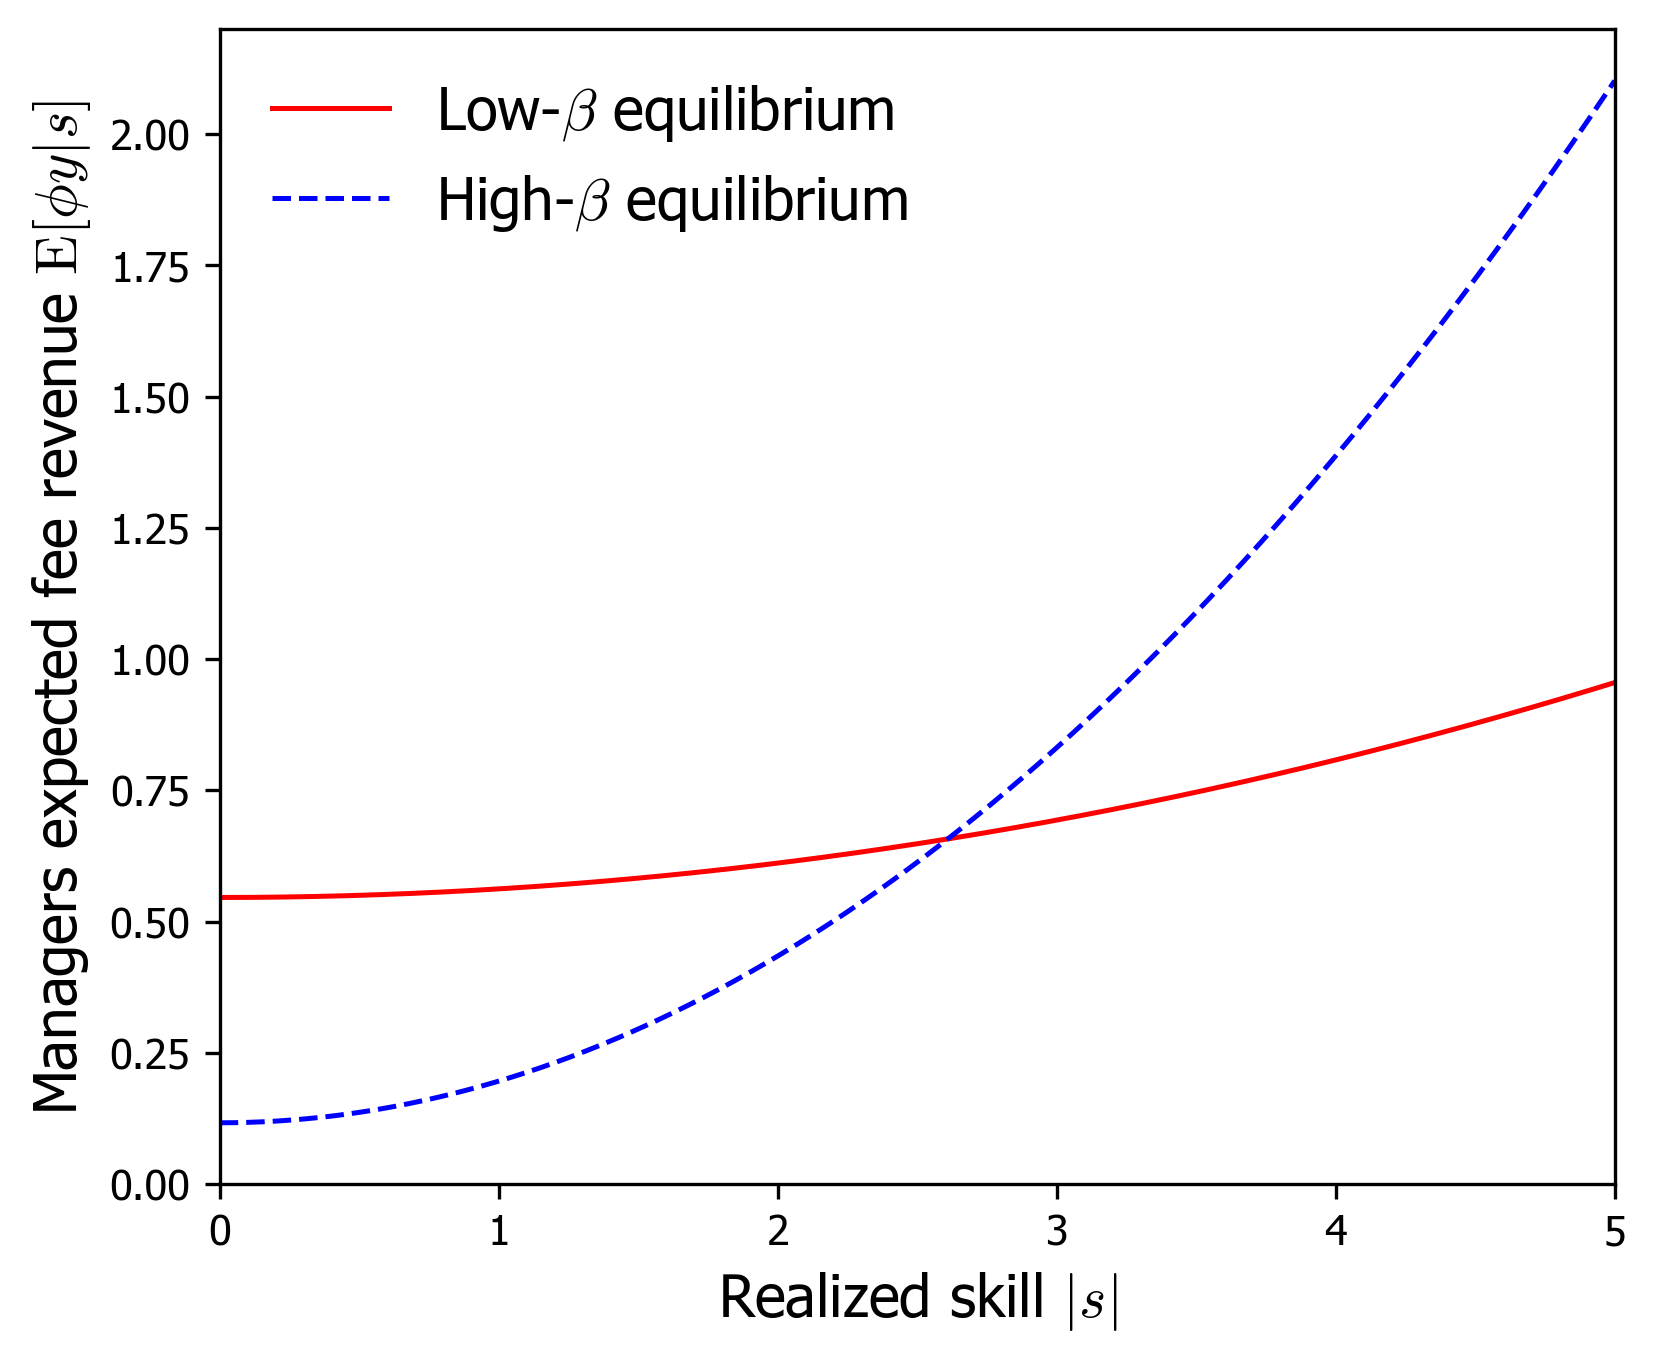
\includegraphics[width=80mm]{./Figures/RelativeWage.png}}
\caption{Skill versus Expected Wage}
\caption*{\footnotesize{Note: The figure plots the manager's expected fee income at the low-$\beta$ equilibrium (solid line) and high-$\beta$ equilibrium (dashed line) for different levels of skill, $|s|$. The parameter values used in the figures are $\omega_{s}=1$, $\omega_{u}=2$, $\omega_{\eta}=38$, and $\theta=27$.}}\label{fig:wageSens}
\end{figure}

Our model provides insights into how skills are reflected in compensation in the fund management industry. As shown in statement \ref{item:5} of Corollary \ref{cor:high_vs_low}, fund investors learn $s$ more precisely in the high-$\beta$ equilibrium than in the low-$\beta$ equilibrium, as the manager demonstrates her skill by trading more intensively. Consequently, in the high-$\beta$ equilibrium, the manager's expected compensation, $\mathrm{E}[\phi y|s]$, becomes more sensitive to her realized skill. As an illustration, Figure \ref{fig:wageSens} plots the manager's expected compensation in relation to her skill in the low- and high-$\beta$ equilibria. In the high-$\beta$ equilibrium, investors' accurate evaluations result in greater pay inequality: low-skilled managers would receive very low compensation, while high-skilled ones are very highly paid. This result corroborates empirical observations, such as those provided by \citet{philippon2012wages} and \citet*{bohm2018since}, highlighting the comparatively large wage inequality in the fund management industry. \citet{celerier2019returns} attribute the source of wage inequality to the scalability of skill, while inequality in our model arises from managers' incentives to attract fund flows through establishing high reputation.

%-------------------------------------------
\subsubsection{Skill and Performance Persistence}\label{sss:skill_persistence}

Do high-skilled managers consistently perform well? Not always: skilled managers may not necessarily outperform less skilled ones. Consider a highly skilled manager and a relatively less skilled one. Since trading profits are increasing in managers' skill $|s|$, the former is expected to achieve higher trading profits than the latter \emph{conditional on} both managers trading at the same intensity $\beta$. However, if their investors believe, for whatever reason, that the skilled manager invests more aggressively than the less skilled one, and managers conform to such beliefs, a high skill level does not translate into performance. This is because the skilled manager, trading at the reputation-driven equilibrium, reveals too much private information to the market maker. Hence, compared to the less skilled manager, who plays the Kyle-like equilibrium, the skilled manager may earn lower expected profits. Figure \ref{fig:perf}  illustrates such a situation.\footnote{The same argument holds for the comparison of the unconditional expected profit, $\mathrm{E}[\pi]$, using skill variance $\omega_{s}$ as an \textit{ex-ante} measure of the skill level.} It plots the expected trading profits (performance) at high- and low-$\beta$ equilibria with different levels of skill, suggesting that a low-skilled manager in the low-$\beta$ equilibrium (point B) outperforms a high-skill manager in the high-$\beta$ equilibrium (point A).

\begin{figure}
\centering
{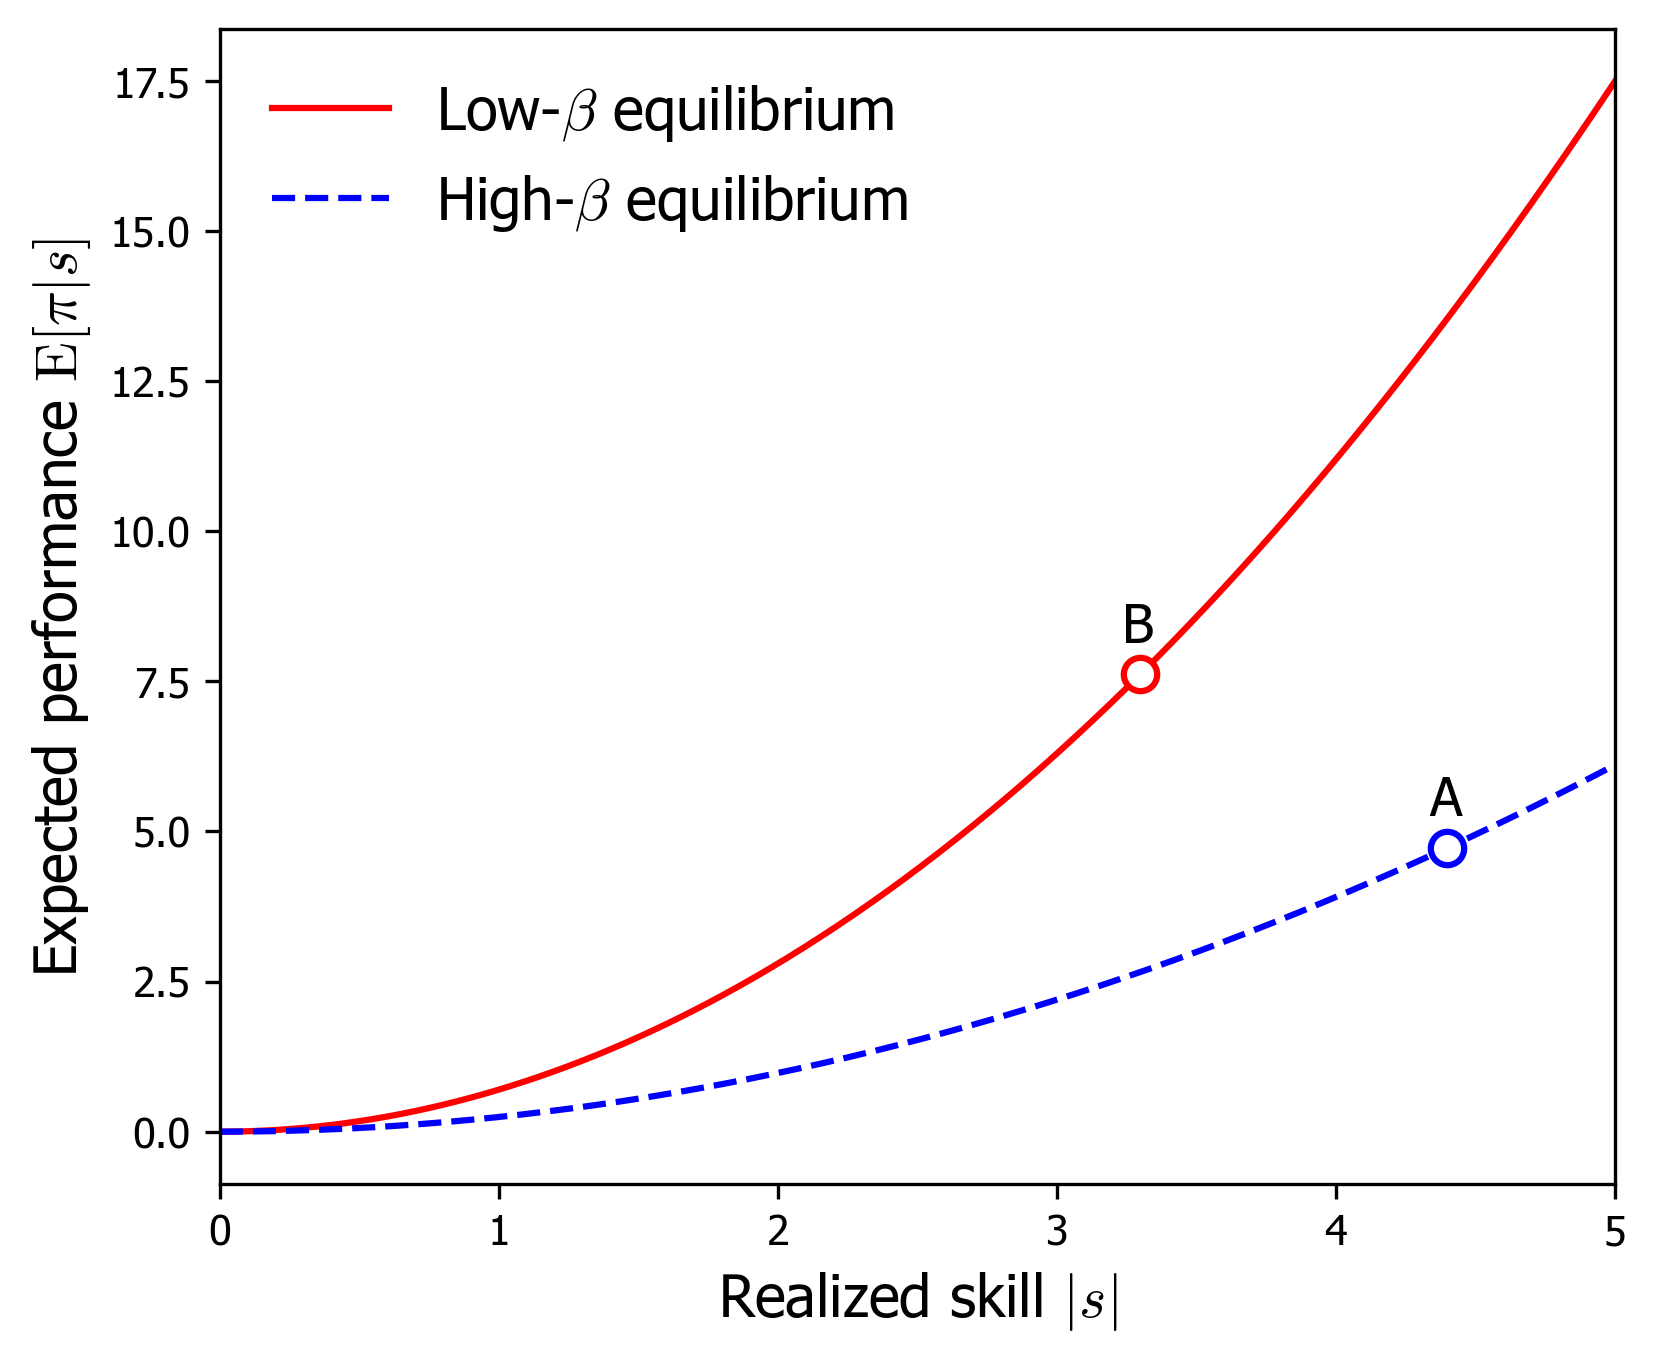
\includegraphics[width=85mm]{./Figures/PerformanceSkillRealized.png}\label{high2}}
\caption{Skill versus Expected Trading Profit}
\caption*{\footnotesize{Note: The figure plots the expected trading profit $\mathrm{E}[\pi]$ at the low-$\beta$ equilibrium (solid line) and the high-$\beta$ equilibrium (dashed line) for different levels of skill $|s|$. The parameter values used in the figure are $\omega_{s}=1$, $\omega_{u}=2$, $\omega_{\eta}=38$, and $\phi=0.02$.}}
\label{fig:perf}
\end{figure}

The empirical literature (e.g., \citealp{jensen1967performance}; \citealp*{busse2010performance}) finds that asset managers do not outperform passive benchmarks on average and, in cross-section, those who outperform cannot do so consistently. While the literature attributes the lack of persistent performance to the lack of skill, our result proposes an alternative explanation. Several studies reconcile the existence of skill with the lack of persistent performance. \citet{berk2004mutual}, for example, argue that skill-based alphas eventually disappear due to competition between investors and decreasing returns to scale at the fund level.\footnote{\citet*{pastor2015scale} document increases in skill in finance and attribute the lack of corresponding increases in performance to decreasing returns to scale at the industry level.} Our model contributes to the understanding of this matter by showing that the absence of a systematic skill-performance relationship could be the result of self-fulfilling multiple equilibria.
